In this chapter, we analyze two proposed idealized models of the TCPC. These models are designed to incorporate key geometric modifications identified as beneficial in reducing energy dissipation, as described in \cite{Rijnberg2018}. These modifications, summarized in Figure~\ref{fig:positive_modifications}, serve as a foundation for investigating the effects of caval offsetting, curving, flaring, and other geometric factors on flow dynamics.

\begin{figure}[H]
	\centering
	\includegraphics[width=0.65\textwidth]{figures/energyloss-en.pdf}
	\caption[Positive Modifications for TCPC]{Key modifications to improve TCPC geometry and reduce energy dissipation: (a) caval offsetting, where the inferior and superior vena cava are misaligned to minimize flow collision; (b) curving, where the conduits are curved to enhance flow alignment; (c) the Y-graft configuration, which splits the flow evenly between outlets; and (d) flaring, where the connections are widened to reduce sharp corners and flow resistance. Adapted from \cite{Rijnberg2018}.}
	\label{fig:positive_modifications}
\end{figure}

\section{The Models}

To systematically evaluate the effects of geometric changes, the models were developed with varying levels of complexity, incorporating different numbers of degrees of freedom. Both models represent idealized TCPC geometries and share the same labeling convention for inlets and outlets. Specifically, the inlets are denoted as $\Gamma^{N}_{\text{in}}$ (top inlet representing the superior vena cava) and $\Gamma^{S}_{\text{in}}$ (bottom inlet representing the inferior vena cava with the conduit). The outlets are labeled as $\Gamma^{W}_{\text{out}}$ (left outlet representing the left pulmonary artery) and $\Gamma^{E}_{\text{out}}$ (right outlet representing the right pulmonary artery). The shared geometric framework, along with labeled boundaries, is illustrated in Figure~\ref{fig:junction schema}.

\begin{figure}[H]
	\centering
	\begin{subfigure}{0.45\textwidth}
		\centering
		\includegraphics[width=0.75\textwidth, trim={0mm -13mm 0mm 0mm}]{figures/3dschema.pdf}
		\caption{3D schematic of the idealized TCPC junction.}
		\label{fig:schema 3d}
	\end{subfigure}\hspace{2mm}
	\begin{subfigure}{0.53\textwidth}
		\centering
		\includegraphics[width=0.99\textwidth, trim={0mm -5mm 0mm 0mm}]{figures/2dschema.pdf}
		\caption{2D schematic of the idealized TCPC junction, highlighting labeled boundaries.}
		\label{fig:schema 2d}
	\end{subfigure}
	\vspace{2mm}
	\caption[Schematic of Idealized TCPC Geometry]{2D and 3D schematic illustrations of the idealized TCPC geometry, showing labeled inlets ($\Gamma^{N}_{\text{in}}$, $\Gamma^{S}_{\text{in}}$) and outlets ($\Gamma^{W}_{\text{out}}$, $\Gamma^{E}_{\text{out}}$).}
	\label{fig:junction schema}
\end{figure}


\subsection{Model 1: Simplified Cylindrical Junction}

The first model represents a basic cylindrical junction, where the bottom vertical cylinder corresponds to the inferior vena cava (IVC), the horizontal cylinder corresponds to the pulmonary artery, and the top vertical cylinder represents the superior vena cava (SVC). The IVC and SVC are connected perpendicularly to the pulmonary artery, creating a cross-like structure. 

Model 1 was chosen because it introduces only one degree of freedom: the vertical offset of the IVC relative to the SVC. This simplicity makes it feasible to sample and evaluate the optimization space exhaustively, providing an opportunity to study the behavior of the objective functions, namely wall shear stress (WSS) and turbulence kinetic energy (TKE), in detail.

\begin{figure}[H]
	\centering
	\includegraphics[width=0.8\textwidth]{figures/krizovatka-obecna.pdf} % Replace with your figure for Model 1
	\caption[Simplified Cylindrical Junction]{Schematic of Model 1: A simplified cylindrical junction with one degree of freedom, the vertical offset of the IVC relative to the SVC.}
	\label{fig:model1_schematic}
\end{figure}

\subsection{Model 2: Complex Geometric Model}

The second model introduces additional complexity by incorporating five degrees of freedom: the vertical offset of the IVC, the angles of connection for both the IVC and SVC to the pulmonary artery, the flaring of the IVC, and the width of the IVC. This model enables a more detailed investigation of the interaction between geometric parameters and hemodynamic efficiency.

Model 2 was selected because its higher complexity allows for greater variations in geometry and, consequently, a potentially larger impact on flow dynamics. However, the increased number of degrees of freedom makes it infeasible to sample the optimization space comprehensively, rendering the model more akin to a "black box" during optimization.

\begin{figure}[H]
	\centering
	\includegraphics[width=0.8\textwidth]{figures/krizovatka-obecna.pdf} % Replace with your figure for Model 2
	\caption[Complex Geometric Model]{Schematic of Model 2: A more complex model with five degrees of freedom—IVC offset, connection angles, flaring, and width of the IVC.}
	\label{fig:model2_schematic}
\end{figure}
